%%%%%%%%%%%%%%%%%%%%%%%%%%%%%%%%%%%%%%%%%
% Journal Article
% LaTeX Template
% Version 1.4 (15/5/16)
%
% This template has been downloaded from:
% http://www.LaTeXTemplates.com
%
% Original author:
% Frits Wenneker (http://www.howtotex.com) with extensive modifications by
% Vel (vel@LaTeXTemplates.com)
%
% License:
% CC BY-NC-SA 3.0 (http://creativecommons.org/licenses/by-nc-sa/3.0/)
%
%%%%%%%%%%%%%%%%%%%%%%%%%%%%%%%%%%%%%%%%%

%----------------------------------------------------------------------------------------
%	PACKAGES AND OTHER DOCUMENT CONFIGURATIONS
%----------------------------------------------------------------------------------------

\documentclass[10pt]{article} % Single column

%\documentclass[twoside,twocolumn]{article} % Two column

\usepackage{blindtext} % Package to generate dummy text throughout this template 

\usepackage[sc]{mathpazo} % Use the Palatino font
\usepackage[T1]{fontenc} % Use 8-bit encoding that has 256 glyphs
\linespread{1.05} % Line spacing - Palatino needs more space between lines
\usepackage{microtype} % Slightly tweak font spacing for aesthetics

\usepackage[spanish]{babel} % Language hyphenation and typographical rules

\usepackage[hmarginratio=1:1,top=32mm,columnsep=20pt]{geometry} % Document margins
\usepackage[hang, small,labelfont=bf,up,textfont=it,up]{caption} % Custom captions under/above floats in tables or figures
\usepackage{booktabs} % Horizontal rules in tables

\usepackage{lettrine} % The lettrine is the first enlarged letter at the beginning of the text

\usepackage{enumitem} % Customized lists
\setlist[itemize]{noitemsep} % Make itemize lists more compact

\usepackage{abstract} % Allows abstract customization
\renewcommand{\abstractnamefont}{\normalfont\bfseries} % Set the "Abstract" text to bold
\renewcommand{\abstracttextfont}{\normalfont\small\itshape} % Set the abstract itself to small italic text

\usepackage{titlesec} % Allows customization of titles
\renewcommand\thesection{\Roman{section}} % Roman numerals for the sections
\renewcommand\thesubsection{\roman{subsection}} % roman numerals for subsections
\titleformat{\section}[block]{\large\scshape\centering}{\thesection.}{1em}{} % Change the look of the section titles
\titleformat{\subsection}[block]{\large}{\thesubsection.}{1em}{} % Change the look of the section titles

\usepackage{fancyhdr} % Headers and footers
\pagestyle{fancy} % All pages have headers and footers
\fancyhead{} % Blank out the default header
\fancyfoot{} % Blank out the default footer
\fancyhead[C]{Sistemas Distribuidos. \textbf{Monica Scheduler}} % Custom header text
\fancyfoot[RO,LE]{\thepage} % Custom footer text

\usepackage{titling} % Customizing the title section

\usepackage{hyperref} % For hyperlinks in the PDF

\usepackage{graphicx} % For images

\usepackage{pifont} % bullets

\usepackage{amsmath}

\usepackage{algpseudocode}

\usepackage{float}
% Keywords command
\providecommand{\keywords}[1]
{
	\small	
	\vspace{0.5em}
	\noindent \textbf{\textit{Palabras clave --- }} #1
}


%----------------------------------------------------------------------------------------
%	TITLE SECTION
%----------------------------------------------------------------------------------------

\setlength{\droptitle}{-4\baselineskip} % Move the title up

\pretitle{\begin{center}\Huge\bfseries} % Article title formatting
	\posttitle{\end{center}} % Article title closing formatting
\title{\normalsize{Sistemas Distribuidos}\\
	\Huge\bfseries Monica Scheduler \\
} % Article title
\author{% 
	% \includegraphics[width=15em]{logo.png}\\
	Laura Victoria Riera P\'erez\\
	Mari\'e del Valle Reyes \vspace{1em} \\
	\small Cuarto a\~no. Ciencias de la Computaci\'on. \\ % institution
	\small Facultad de Matem\'atica y Computaci\'on, Universidad de La Habana, Cuba \\ % institution
}
\date{\footnotesize \today } % Leave empty to omit a date


% Abstract configurations
\renewenvironment{abstract}
{\small
	\begin{center}
		\bfseries \abstractname\vspace{-.5em}\vspace{0pt}
	\end{center}
	\list{}{
		\setlength{\leftmargin}{1.5cm}%
		\setlength{\rightmargin}{\leftmargin}%
	}%
	\item\relax}
{\endlist}

\usepackage{amsthm}
\usepackage{amssymb}
\usepackage{todonotes} % \TODO
\usepackage{listings} % Code listings
\usepackage{xcolor}

\definecolor{backcolour}{rgb}{0.95,0.95,0.92}

\newcommand{\csl}[1]{\colorbox{backcolour}{\texttt{#1}}}

\newcommand{\imgcaption}[2]{\tiny \textbf{Figura #1.} #2.}

\newcommand{\mgc}[2][]{\colorbox{backcolour}{\texttt{\_\_#2\_\_#1}}}

\newcommand{\mgccapt}[1]{\texttt{\_\_#1\_\_}}

\newtheorem{thm}{Teorema}
\newtheorem{mydef}{Definici\'on}%[section]
\newtheorem{lem}{Lema}
\newtheorem{fig}{\scriptsize{Figura}}


\renewcommand{\qedsymbol}{\rule{0.7em}{0.7em}}

% Hyperlinks configurations
\hypersetup{
	colorlinks=true,
	linkcolor=black,
	filecolor=magenta,      
	urlcolor=cyan,
	pdftitle={Overleaf Example},
	pdfpagemode=FullScreen,
}

%----------------------------------------------------------------------------------------

\begin{document}
	
	\bibliographystyle{ieeetr}
	
	% Print the title
	\maketitle
	
	%----------------------------------------------------------------------------------------
	%	ARTICLE CONTENTS
	%----------------------------------------------------------------------------------------
	
	\section*{Repositorio del proyecto}
	
	\begin{center}
		\href{https://github.com/computer-science-crows/monica-scheduler}{https://github.com/computer-science-crows/monica-scheduler}
	\end{center}

	\section{Introducción}
	
	El tiempo es un recurso invaluable y su gestión eficiente es esencial para la productividad y el bienestar personal. Una estrategia comúnmente utilizada para la gestión del tiempo es el uso de una agenda. Sin embargo, en muchas ocasiones, es necesario coordinar dicha agenda con otras personas para llevar a cabo actividades conjuntas. Este proceso implica la identificación de horarios compartidos y la detección de intervalos de tiempo libres. Además, estas planificaciones pueden verse alteradas por eventos imprevistos que requieren asistencia, lo que conlleva la necesidad de modificar la agenda nuevamente.
	
	Para abordar estos desafíos, este proyecto propone la creación de una agenda electrónica distribuida como herramienta de gestión del tiempo para eventos personales o grupales. El sistema se diseñó e implementó como un sistema distribuido, utilizado la Tabla Hash Distribuida (DHT) de Kademlia para la gestión de datos.
	
	\section{Requerimientos}
	
	Este proyecto consiste en crear una agenda distribuida como herramienta de gestión del tiempo para eventos personales o grupales. Los requisitos clave para este sistema son:
	
	\begin{itemize}
		\item \textbf{Arquitectura Distribuida}: El sistema debe ser diseñado e implementado como un sistema distribuido. Esto significa que el sistema debe ser capaz de funcionar en múltiples máquinas mientras se presenta a los usuarios como un sistema coherente único.
		
		\item \textbf{Mecanismo de Autenticación e Identificación}: El sistema debe ser capaz de autenticar e identificar a cada usuario. Esto asegura que solo los usuarios autorizados puedan acceder al sistema y realizar ciertas acciones.
		
		\item \textbf{Formación de Grupos}: El sistema debe permitir la creación de grupos, ya sean jerárquicos o no jerárquicos. Esto significa que los usuarios deben poder crear y gestionar grupos dentro del sistema de manera flexible.
		
		\item \textbf{Citas Grupales}: El sistema debe admitir la creación de citas grupales. Si se utiliza un grupo jerárquico, una cita creada por un superior debe aparecer automáticamente en las agendas de todos los miembros del grupo. Para grupos no jerárquicos, todos los miembros deben aceptar la cita para que se confirme.
		
		\item \textbf{Actualizaciones Automáticas de la Agenda}: Cuando se crea, modifica o elimina una cita, los cambios deben reflejarse automáticamente en las agendas de los usuarios relevantes.
		
		\item \textbf{Identificación de Conflictos}: El sistema debe ser capaz de identificar conflictos en las agendas locales. Por ejemplo, si un usuario tiene programadas dos citas al mismo tiempo, el sistema debe señalar esto como un conflicto.
		
	\end{itemize}
	
	\section{Arquitectura del Sistema}
	
	El sistema se compone de cuatro partes fundamentales: CLI, capa de negocio, capa que conecta la l\'ogica con la red y la red con los datos.
	
	\begin{center}
		\begin{figure}[h]
			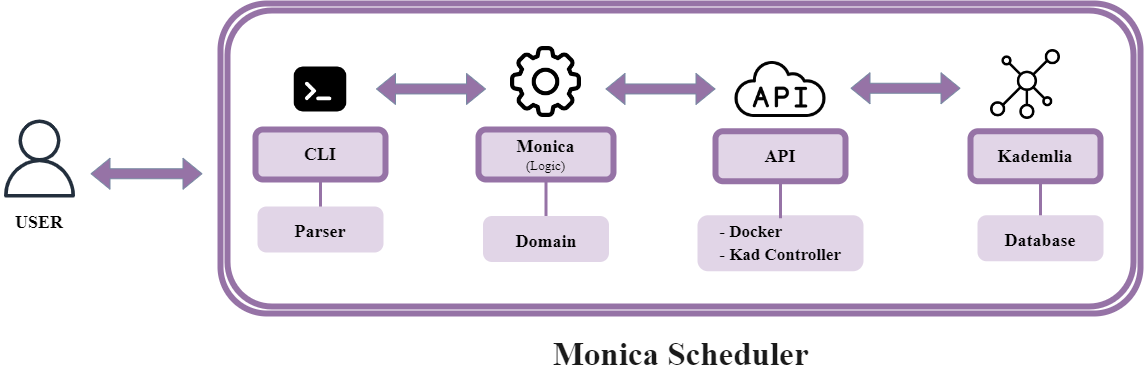
\includegraphics[scale=0.4]{esquema}
			\caption{Esquema de flujo del sistema.}
			\label{esquema}
		\end{figure}
		
	\end{center}
	
	\subsection{CLI}
	
	Para facilitar la presentación y prueba del sistema, se implementó una interfaz de línea de comandos (CLI, por sus siglas en inglés) que permite a los usuarios interactuar con el sistema de manera flexible y eficiente. En su desarrollo se utilizó el módulo \textit{\textbf{argparse}} de Python para analizar y procesar cada línea de comando ingresada por los usuarios.
	
	La CLI proporciona una variedad de comandos que los usuarios pueden ejecutar para realizar diferentes acciones en el sistema. Al ejecutar el sistema e ingresar el comando \texttt{-h} o \texttt{---}\texttt{help}, se muestra una lista completa de los comandos disponibles junto con su descripción correspondiente. Esta funcionalidad brinda a los usuarios una referencia rápida y fácil de los comandos admitidos, lo que facilita la interacción con el sistema.
	
	Gracias al uso del módulo argparse, se implementa una lógica robusta para analizar y manejar los argumentos de la línea de comandos. Esto incluye la validación de los argumentos ingresados y la ejecución de las acciones correspondientes en función de los comandos proporcionados. Los usuarios pueden proporcionar los argumentos requeridos y opcionales de manera ordenada y estructurada, lo que mejora la experiencia de uso y evita posibles errores de entrada.
	
	\subsection{Monica}	
	
	La capa de lógica de negocio desempeña un papel fundamental en la implementación y gestión de las reglas y procesos específicos del sistema. Dentro de esta capa, se llevaron a cabo diversas actividades clave para garantizar el correcto funcionamiento y cumplimiento de los requisitos del negocio.
	
	Una de las actividades esenciales fue la validación y verificación de datos. Esto implic\'o asegurarse de que los datos recibidos fueran válidos y cumplieran con las reglas establecidas. Se realizaron comprobaciones exhaustivas para garantizar la integridad y calidad de los datos antes de procesarlos, evitando posibles inconsistencias o errores en el sistema. Para la coordinaci\'on de procesos del sistema se tuvieron que orquestar y sincronizar diferentes operaciones y componentes para garantizar la correcta secuencia y flujo de las tareas, asegurando que cada paso se realizara en el momento adecuado y en conformidad con las dependencias y restricciones establecidas. Adem\'as, se manejaron adecuadamente las excepciones, capturándolas, registrándolas y tomando las medidas necesarias para mitigar su impacto, as\'i como se proporcionaron mensajes de error claros y significativos para informar al usuario sobre las incidencias y facilitar su resolución.
	
	
	\subsubsection{Dominio}	
	El dominio de nuestro sistema se centra en la gestión colaborativa de eventos y actividades entre múltiples usuarios. En \'el se identifican cuatro entidades principales: User (Usuario), Request (Petición), Event (Evento) y Workspace.
	\begin{itemize}
		\item \textbf{User:} Representa a los usuarios de la aplicación de agenda distribuida. Cada usuario puede tener atributos como nombre, alias y contraseña, los cuales se utilizan para identificar y autenticar a los usuarios en el sistema.
		\item \textbf{Request:} Representa las peticiones realizadas dentro de la aplicación. Estas peticiones pueden ser de distintos tipos y se envían entre usuarios para realizar acciones específicas. Los atributos y relaciones de la entidad Request se detallan en la Figura [\ref{merx}].
		\item \textbf{Event:} Representa los eventos o actividades programadas en la agenda distribuida. Cada evento puede tener atributos como título, fecha, lugar, hora de inicio y hora de finalización, que permiten identificar y organizar las diferentes actividades en el sistema.
		\item \textbf{Workspace:} Representa los espacios de trabajo colaborativo en los cuales se comparte la agenda distribuida. Cada workspace puede tener un nombre asociado y permite agrupar a los usuarios y eventos relacionados.
	\end{itemize}

	Las relaciones y atributos específicos de las entidades  se encuentran detallados en la Figura [\ref{merx}], proporcionando una representación visual que muestra cómo se conectan y se relacionan estas entidades dentro del dominio de la aplicación de agenda distribuida.
	


	\begin{center}
		\begin{figure}[h]
			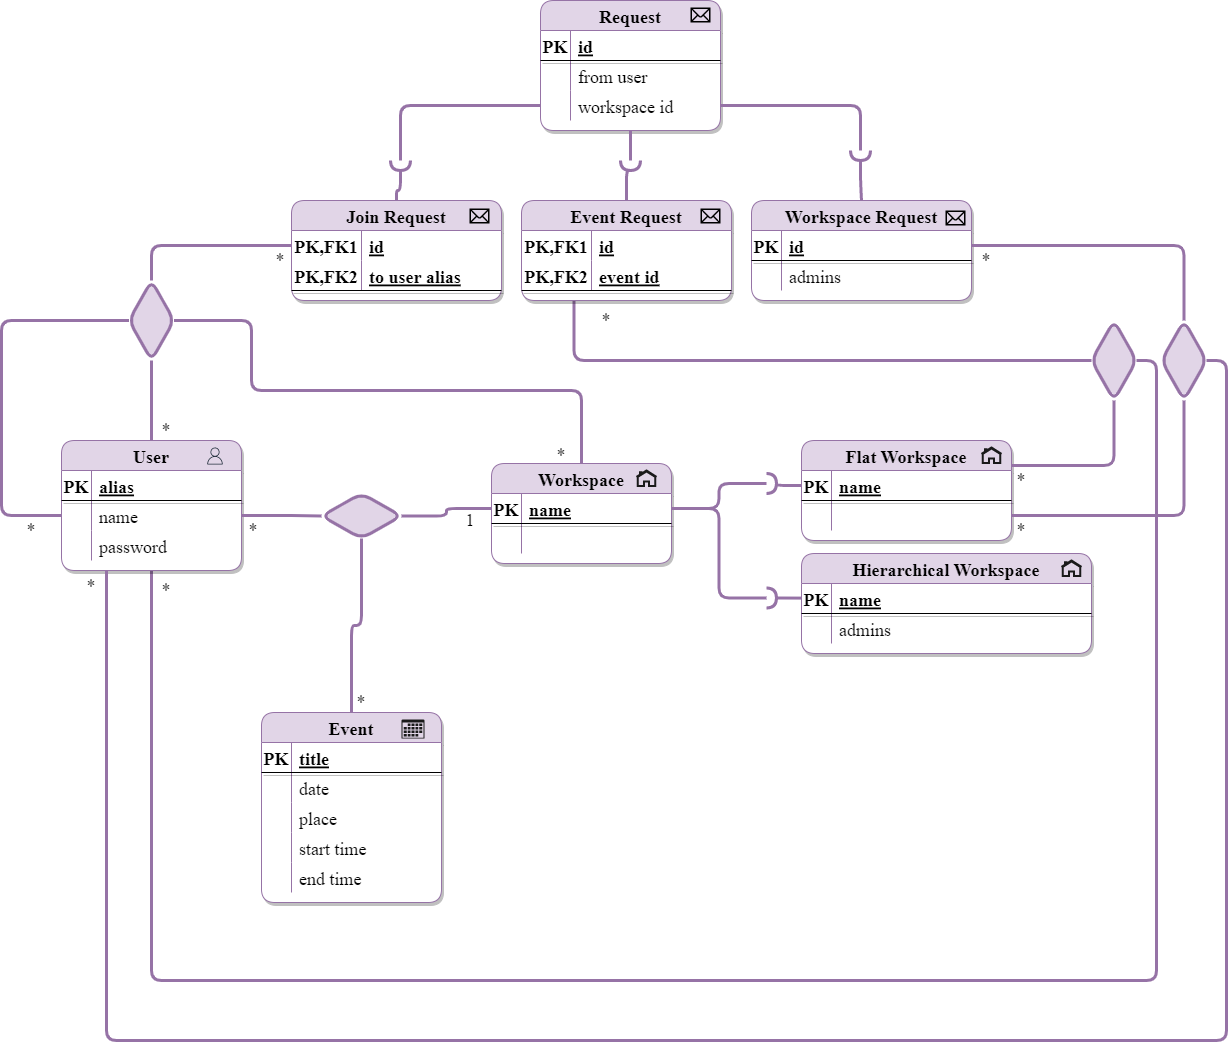
\includegraphics[scale=0.35]{modelo-merx}
			\caption{Diagrama entidad-relaci\'on del problema agenda distribuida.}
			\label{merx}
		\end{figure}
		
	\end{center}

	 
	\subsection{API}
	
	Esta capa se encarga de conectar la l\'ogica de negocio con la red de datos. La clase API, primeramente se encarga de construir la imagen de docker y levantar la red de Kademlia con una cantidad de nodos igual a dos, creando un container por cada uno. Tiene cinco m\'etodos fundamentales: build\_image (construye la imagen de docker), create\_servers(crea contenedores y por cada uno levanta un servidor de la red), remove\_servers (para un n\'umero random de contenedores), get\_value (dada una llave levanta un contenedor temporal que se conecta a la red para obtener el valor correspondiente y al obtenerlo lo para) y set\_value (dada una llave y un valor levanta un contenedor temporal que se conecta a la red para obtener el establecer el valor correspondiente en la llave especificada, y lugo para el container).
	
	\subsection{Red de Kademlia}
	
	Kademlia \cite{kad} es un protocolo descentralizado utilizado en redes peer-to-peer (P2P) para el almacenamiento y recuperación eficiente de información. Los nodos en la red se representa mediante una identificación única llamada ID de nodo que se deriva del valor hash de una clave pública criptográfica. El protocolo utiliza una estructura de árbol binario conocida como ''árbol de cubetas'' para organizar los nodos en la red. Cada nodo mantiene una tabla de enrutamiento que contiene información sobre otros nodos en la red y su cercanía en el espacio de direcciones. Esta tabla se divide en ''cubetas'' que agrupan nodos con direcciones similares. Cuando un nodo necesita buscar o almacenar información, realiza consultas a través de la red utilizando la distancia de XOR entre los ID de nodo como criterio de enrutamiento. Esto permite un enrutamiento eficiente hacia los nodos más cercanos al ID de destino.
	
	El protocolo es conocido por su resistencia a fallos y su capacidad para adaptarse a cambios en la red, como nodos que se unen o abandonan. También es escalable, lo que significa que puede funcionar eficientemente en redes P2P grandes con millones de nodos.		
	

	
	\subsubsection{Implementaci\'on}
	
	En la implementación de la red Kademlia, se utiliza un algoritmo basado en DHT (Distributed Hash Table) para realizar búsquedas en la red. Este algoritmo busca los \textit{k} nodos más cercanos a una clave específica en términos de distancia XOR. El proceso comienza seleccionando $\alpha$ contactos de las \textit{k} cubetas que contienen los nodos más cercanos a la clave buscada. Luego, se envían mensajes asincrónicos a estos contactos para obtener información sobre la clave. Cada contacto activo devuelve información que ayuda a acercarse al nodo objetivo. Este proceso se repite hasta encontrar el nodo deseado.
	
	
	Cuando un nuevo nodo desea unirse a la red de Kademlia, se utiliza un mecanismo de \textit{broadcast}. El nuevo nodo envía un mensaje de broadcast y espera activamente a que alg\'un nodo responda a su solicitud. Los nodos que reciben el mensaje pueden decidir responder al nuevo nodo proporcionando su dirección IP. Una vez que se recibe la respuesta, el nuevo nodo puede utilizar la información proporcionada para establecer una conexión con la red y actualizar su tabla de enrutamiento para incluir a los nodos con los que ha establecido comunicación. A su vez,  los nodos existentes actualizan sus tablas de enrutamiento para incluir al nuevo nodo.
	
	% Sin embargo, los vecinos más cercanos del nuevo nodo no comparten automáticamente todos sus datos. En cambio, el nuevo nodo participa en la red almacenando y recuperando datos según lo soliciten otros nodos. De esta manera, los datos se almacenan y recuperan según sea necesario, basándose en las solicitudes de otros nodos de la red.
	
	Para el almacenamiento de datos, se utilizó la biblioteca \texttt{dictdatabase}, la cual proporciona métodos para obtener y guardar datos en archivos con formato JSON. La clave de los valores se genera a partir del SHA1 del identificador del objeto. Cada vez que se modifica el objeto, se actualiza el valor asociado a dicha llave en la base de datos.
	
	Se consideró otra opción que consistía en aplicar el algoritmo SHA1 a toda la información que encapsula el objeto, lo que generaría una nueva clave cada vez que se modifica el objeto. Sin embargo, esta opción aumentaría la cantidad de datos almacenados y sería difícil mantener la consistencia de la mayoría de los datos, ya que se requeriría cambiar la clave antigua por la nueva en cada objeto que la almacene. Por lo tanto, se decidió utilizar el enfoque anteriormente mencionado para asegurar una gestión eficiente y coherente de los datos almacenados.
	
	
	
	
	
	\section{Docker}
	
	Para simular distintos servidores en un sistema distribuido, utilizamos Docker. Cada contenedor Docker puede considerarse como un nodo en el sistema distribuido, capaz de ejecutar su propio sistema operativo, tener su propia configuración de red y ejecutar las aplicaciones como si estuviera en una máquina separada. Esto permite simular un sistema distribuido en una sola máquina física, lo que facilita el desarrollo y las pruebas del sistema.
	

	
	\begin{thebibliography}
		a
		\bibitem{kad} Maymounkov, P., Mazières, D. (2002). \textit{Kademlia: A Peer-to-Peer Information System Based on the XOR Metric.} In: Druschel, P., Kaashoek, F., Rowstron, A. (eds) Peer-to-Peer Systems. IPTPS 2002. Lecture Notes in Computer Science, vol 2429. Springer, Berlin, Heidelberg.
	\end{thebibliography}
\end{document}


